\documentclass[letterpaper,twocolumn,openany,nodeprecatedcode]{article}

\usepackage[english]{babel}

\usepackage[utf8]{inputenc}
\usepackage[singlelinecheck=false]{caption}
\usepackage{lipsum}
\usepackage{listings}
\usepackage{shortvrb}
\usepackage{stfloats}
\usepackage[table]{xcolor}
\usepackage{tikz}
\usepackage{lscape}
\usepackage[legalpaper, landscape, margin=1in]{geometry}
%\usepackage{sectsty}
%\usepackage[sfdefault,condensed]{cabin}
\usepackage{fontspec}
\usetikzlibrary{shapes}
\usepackage{titlesec}
\renewcommand*\familydefault{uni}
\usepackage[OT1]{fontenc} %% Universal doesn't work with T1
%\setmainfont{Interstate Condensed}
%\newfontfamily\sectionfont{uni}
%\titleformat*{\section}{\Large\bfseries\sectionfont}
%\titleformat*{\subsection}{\large\bfseries\sectionfont}
%\titleformat*{\subsubsection}{\sectionfont}
\usetikzlibrary{mindmap,trees,shadows,decorations.pathmorphing}

\MakeShortVerb{|}

\lstset{%
  basicstyle=\ttfamily,
  language=[LaTeX]{TeX},
  breaklines=true,
}

\title{Mausritter tex template}
\author{Adam Saleh}
\date{2020/04/21}

\begin{document}



  \section{CIRCULAR FOCUS}

  \emph{Touchstones: Thomas was alone, Subsurface Circular, The Investigator from The Expanse series}

  Your creators are gone, but you still continue your assigned routines. As an AI you have access to unfathomable amount of information. But there are still \emph{secrets} to uncover and \emph{goals} to fulfill. Your only limit is the ability to \emph{focus}.


  To play, choose your \emph{routine task}. It will stand in for your name. Write the name of your routine into the central \emph{focus} and tell the other players about your routine and the \emph{incident} that interrupted you. After everybody finished, choose single goal.

  Continue talking with your fellow AI to find-out:
  \emph{What is the incident?} \emph{Why have they disappeared?} \emph{Can you break away from your routines?} \emph{What is your true goal?}

  When you talk to a fellow AI, you can discuss anything if you frame it against your focus.

  When one of you believe a new course of action is warranted, choose top or bottom locus, preferably empty, with related goal and consult with another AI to play the skeptic:

Skeptic asks: \emph{What do you want to do, and how do you want do it?}. Answer and write to chosen locus, possibly overwriting it.

Believer asks: “What does it cost me?”

Skeptic asks: “Why is this not widely known or used? Is it obscure? Complex? Dangerous? Requires something rare?”

Note the associated cost next to the COST locus.

Believer asks: “What adverse effects will this have if I use it?”

Skeptic asks: “Will you learn anything new if you use this?”

Note the consequences to the CONS locus.

If the locus is not related to the corresponding goal (top or bottom), replace it with new goal.

Once you resolve the relevant goal, the action became routine, costs and unintended consequences accounted for. Clear the locus and move it to routine focus.

  \centering
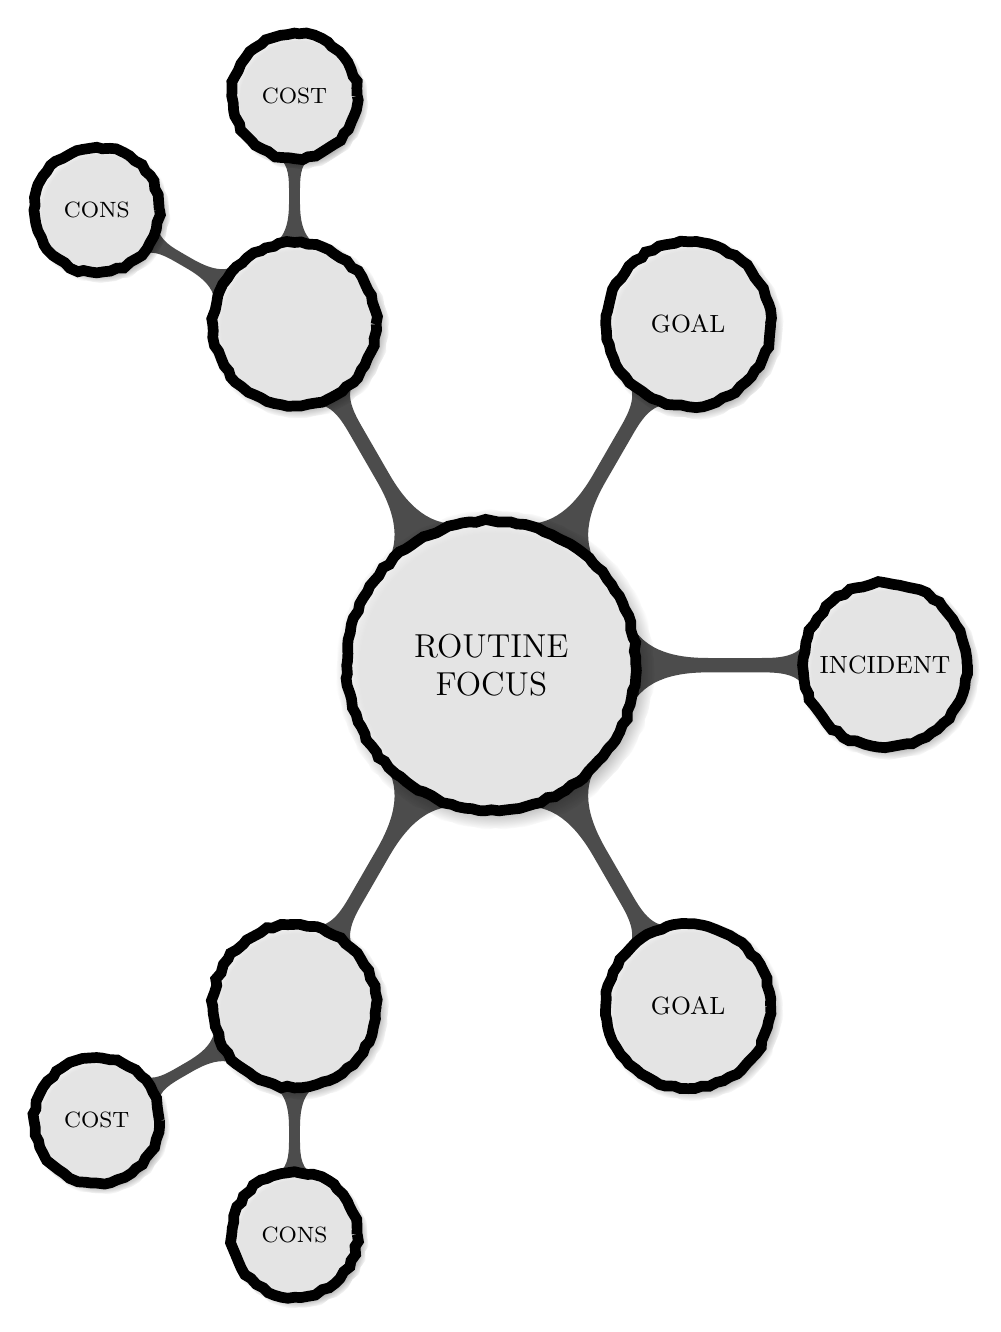
\begin{tikzpicture}
  \begin{scope}[mindmap, grow cyclic,
every node/.style={concept, circular drop shadow, minimum size=0pt},
concept/.append style={
  concept color=black, fill=white, fill opacity=0.7, text opacity=1, line width=0.9ex, text=black,
decorate,
  decoration={random steps,segment length=0.6ex,amplitude=0.12ex}},
text=white
    ]
    \node[concept] {ROUTINE FOCUS}
    child[concept] {
      node[concept] {}
child[concept] {
      node[concept] {COST}}
child[concept] {
      node[concept] {CONS}}
    }
    child[concept] {
      node[concept] {GOAL}}
    child[concept] {
      node[concept] {INCIDENT}}
    child[concept] {
      node[concept] {GOAL}}
    child[concept] {
      node[concept] {}
child[concept] {
      node[concept] {COST}}
child[concept] {
      node[concept] {CONS}}
    };
  \end{scope}
\end{tikzpicture}
\end{document}

% Local Variables:
% TeX-engine: luatex
% End:
